\documentclass[a4paper,12pt]{article}
\usepackage{jheppub}
\usepackage{taro}
\usepackage{booktabs}

\title{Riemann Surfaces}

\author[a]{Taro V. Brown}

\affiliation[a]{Department of Physics, UC Davis, One Shields Avenue, Davis, CA 95616, USA }


% e-mail addresses: one for each author, in the same order as the authors
\emailAdd{tvbrown@ucdavis.edu}


\abstract{}

\begin{document} 
\maketitle
\flushbottom
\newpage
\section{3 point amplitudes bootstrapping}
	Take some open set $U$ in the complex plane and a function $f$ which takes complex variables $z$ and maps them to $\omega=f(z)$ in the open domain $V$
\begin{figure}
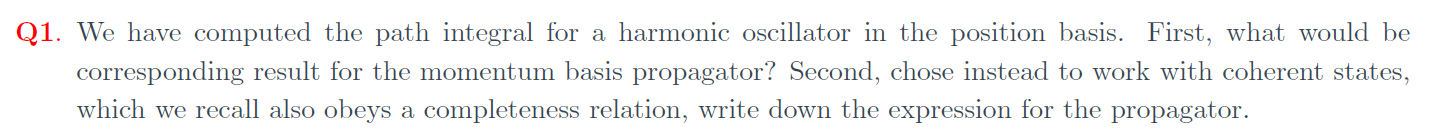
\includegraphics[width=8cm]{1.PNG}
\end{figure}
%%%%%%%%%%%%%%%%%%%%%%%%%%%%%%%%%%%%%%%%%%%%%%%%%%%%%%%%%%%%%%%%%%%%%%%%
\begin{thebibliography}{99}

%\cite{Bjerrum-Bohr:2013bxa}
\bibitem{Bjerrum-Bohr:2013bxa}
N.~E.~J.~Bjerrum-Bohr, J.~F.~Donoghue and P.~Vanhove,
``On-shell Techniques and Universal Results in Quantum Gravity,''
JHEP \textbf{02} (2014), 111
doi:10.1007/JHEP02(2014)111
[arXiv:1309.0804 [hep-th]].
%83 citations counted in INSPIRE as of 21 Aug 2020

%\fi
\end{thebibliography}
\end{document}

